\documentclass{llncs}
%%%%%%%%%%%%%%%%%%%%%%%%%%%%%%%%%%%%%%%%%%%%%%%%%%%%%%%%%%%
%% package sillabazione italiana e uso lettere accentate
\usepackage[english]{babel}
\usepackage[T1]{fontenc}
\usepackage[utf8]{inputenc}
%%%%%%%%%%%%%%%%%%%%%%%%%%%%%%%%%%%%%%%%%%%%%%%%%%%%%%%%%%%%%

\usepackage{url}
\usepackage{xspace}
\usepackage{listings}
\usepackage{xcolor}
\usepackage{textcomp}

\makeatletter
%%%%%%%%%%%%%%%%%%%%%%%%%%%%%% User specified LaTeX commands.
\usepackage{manifest}

\makeatother


%%%%%%%
 \newif\ifpdf
 \ifx\pdfoutput\undefined
 \pdffalse % we are not running PDFLaTeX
 \else
 \pdfoutput=1 % we are running PDFLaTeX
 \pdftrue
 \fi
%%%%%%%
 \ifpdf
 \usepackage[pdftex]{graphicx}
 \else
 \usepackage{graphicx}
\usepackage{caption}
\usepackage{listings}
 \fi
%%%%%%%%%%%%%%%
 \ifpdf
 \DeclareGraphicsExtensions{.pdf, .jpg, .tif}
 \else
 \DeclareGraphicsExtensions{.eps, .jpg}
 \fi
%%%%%%%%%%%%%%%

\newcommand{\java}{\textsf{Java}}
\newcommand{\contact}{\emph{Contact}}
\newcommand{\corecl}{\texttt{corecl}}
\newcommand{\medcl}{\texttt{medcl}}
\newcommand{\msgcl}{\texttt{msgcl}}
\newcommand{\android}{\texttt{Android}}
\newcommand{\dsl}{\texttt{DSL}}
\newcommand{\jazz}{\texttt{Jazz}}
\newcommand{\rtc}{\texttt{RTC}}
\newcommand{\ide}{\texttt{Contact-ide}}
\newcommand{\xtext}{\texttt{XText}}
\newcommand{\xpand}{\texttt{Xpand}}
\newcommand{\xtend}{\texttt{Xtend}}
\newcommand{\pojo}{\texttt{POJO}}
\newcommand{\junit}{\texttt{JUnit}}

\newcommand{\action}[1]{\texttt{#1}\xspace}
\newcommand{\code}[1]{{\small{\texttt{#1}}}\xspace}
\newcommand{\codescript}[1]{{\scriptsize{\texttt{#1}}}\xspace}

% Cross-referencing
\newcommand{\labelsec}[1]{\label{sec:#1}}
\newcommand{\xs}[1]{\sectionname~\ref{sec:#1}}
\newcommand{\xsp}[1]{\sectionname~\ref{sec:#1} \onpagename~\pageref{sec:#1}}
\newcommand{\labelssec}[1]{\label{ssec:#1}}
\newcommand{\xss}[1]{\subsectionname~\ref{ssec:#1}}
\newcommand{\xssp}[1]{\subsectionname~\ref{ssec:#1} \onpagename~\pageref{ssec:#1}}
\newcommand{\labelsssec}[1]{\label{sssec:#1}}
\newcommand{\xsss}[1]{\subsectionname~\ref{sssec:#1}}
\newcommand{\xsssp}[1]{\subsectionname~\ref{sssec:#1} \onpagename~\pageref{sssec:#1}}
\newcommand{\labelfig}[1]{\label{fig:#1}}
\newcommand{\xf}[1]{\figurename~\ref{fig:#1}}
\newcommand{\xfp}[1]{\figurename~\ref{fig:#1} \onpagename~\pageref{fig:#1}}
\newcommand{\labeltab}[1]{\label{tab:#1}}
\newcommand{\xt}[1]{\tablename~\ref{tab:#1}}
\newcommand{\xtp}[1]{\tablename~\ref{tab:#1} \onpagename~\pageref{tab:#1}}
% Category Names
\newcommand{\sectionname}{Section}
\newcommand{\subsectionname}{Subsection}
\newcommand{\sectionsname}{Sections}
\newcommand{\subsectionsname}{Subsections}
\newcommand{\secname}{\sectionname}
\newcommand{\ssecname}{\subsectionname}
\newcommand{\secsname}{\sectionsname}
\newcommand{\ssecsname}{\subsectionsname}
\newcommand{\onpagename}{on page}

\newcommand{\xauthA}{Alessio Tonioni}
\newcommand{\xauthB}{NameB StudentB}
\newcommand{\xauthC}{NameC StudentC}
\newcommand{\xfaculty}{Faculty of Engineering}
\newcommand{\xunibo}{Alma Mater Studiorum -- University of Bologna}
\newcommand{\xaddrBO}{viale Risorgimento 2}
\newcommand{\xaddrCE}{via Venezia 52}
\newcommand{\xcityBO}{40136 Bologna, Italy}
\newcommand{\xcityCE}{47023 Cesena, Italy}

%
% Comments
%
%%% \newcommand{\todo}[1]{\bf{TODO:}\emph{#1}}


%----------------JavaScript highlighting--------------
\lstdefinelanguage{JavaScript}{
  keywords={typeof, new, true, false, catch, function, return, null, catch, switch, var, if, in, while, do, else, case, break},
  keywordstyle=\color{blue}\bfseries,
  ndkeywords={class, export, boolean, throw, implements, import, this},
  ndkeywordstyle=\color{darkgray}\bfseries,
  identifierstyle=\color{black},
  sensitive=false,
  comment=[l]{//},
  morecomment=[s]{/*}{*/},
  commentstyle=\color{purple}\ttfamily,
  stringstyle=\color{red}\ttfamily,
  morestring=[b]',
  morestring=[b]"
}

\lstset{
   language=JavaScript,
   backgroundcolor=\color{lightgray},
   extendedchars=true,
   basicstyle=\footnotesize\ttfamily,
   showstringspaces=false,
   showspaces=false,
   numbers=left,
   numberstyle=\footnotesize,
   numbersep=9pt,
   tabsize=2,
   breaklines=true,
   showtabs=false,
   captionpos=b
}

%-----------------------------Codice disegno--------------------------
\lstset{ %
  backgroundcolor=\color{white},   % choose the background color; you must add \usepackage{color} or \usepackage{xcolor}
  basicstyle=\footnotesize,        % the size of the fonts that are used for the code
  breakatwhitespace=false,         % sets if automatic breaks should only happen at whitespace
  breaklines=true,                 % sets automatic line breaking
  captionpos=b,                    % sets the caption-position to bottom
  commentstyle=\color{green},      % comment style
  deletekeywords={...},            % if you want to delete keywords from the given language
  escapeinside={\%*}{*)},          % if you want to add LaTeX within your code
  extendedchars=true,              % lets you use non-ASCII characters; for 8-bits encodings only, does not work with UTF-8
  frame=single,                    % adds a frame around the code
  keepspaces=true,                 % keeps spaces in text, useful for keeping indentation of code (possibly needs columns=flexible)
  keywordstyle=\color{blue},       % keyword style
  morekeywords={*,...},            % if you want to add more keywords to the set
  numbers=left,                    % where to put the line-numbers; possible values are (none, left, right)
  numbersep=5pt,                   % how far the line-numbers are from the code
  numberstyle=\tiny\color{gray},   % the style that is used for the line-numbers
  rulecolor=\color{black},         % if not set, the frame-color may be changed on line-breaks within not-black text (e.g. comments (green here))
  showspaces=false,                % show spaces everywhere adding particular underscores; it overrides 'showstringspaces'
  showstringspaces=false,          % underline spaces within strings only
  showtabs=false,                  % show tabs within strings adding particular underscores
  stepnumber=1,                    % the step between two line-numbers. If it's 1, each line will be numbered
  stringstyle=\color{red},         % string literal style
  tabsize=2,                       % sets default tabsize to 2 spaces
  title=\lstname                   % show the filename of files included with \lstinputlisting; also try caption instead of title
}

\begin{document}

\title{Software Engineering\\
 progetto "PEdestrian LIght CONtroller"}

%%% \author{\xauthA \and \xauthB}
\author{\xauthA}

\institute{%
%%%  \xunibo\\\xaddrCE, \xcityCE\\\email{\{nameA.studentA, nameB.studentB\}@studio.unibo.it}
  \xunibo\\\xaddrBO, \xcityBO\\\email\ alessio.tonioni@studio.unibo.it
}

\maketitle

%% \begin{abstract}
%% \footnotesize
%%This a Latex template to be used for the reports of Software Engineering.
%%\keywords{Software engineering, managed software development, reports, ....}
%%\end{abstract}

%%% \sloppy

%===========================================================================
\section{Introduction}
\labelsec{intro}
Come caso di studio si analizzi un sistema di gestione di un semaforo per automobili e pedoni.
Il sistema verrà modellato come un automa a stati finiti; per testare la validità dell'analisi si realizzi un prototipo del sistema nella maniera più semplice e veloce possibile.\\
Valutare quindi la semplicit\'a di realizzazione, il grado di riutilizzo e l'estendibilit\'a del prototipo. 
%===========================================================================

%===========================================================================
\section{Vision}
\labelsec{Vision}
Una volta realizzata correttamente la modellazione del sistema, dovremmo essere in grado di realizzare senza alcuno sforzo o perdita di tempo un sistema che concretizzi il comportamento descritto in fase di analisi e che possa essere portato rapidamente in ambienti eterogenei e distribuiti. 
%===========================================================================

%===========================================================================
\section{Goals}
\labelsec{Goals}
Realizzare la modellazione e un prototipo di un sistema di gestione di un incrocio caratterizzato da un semaforo per auto e uno pedonale munito di prenotazione. Cercare di identificare una metodologia per mappare i concetti espressi in fase di analisi in un'implementazione funzionante.
%===========================================================================

%===========================================================================
\section{Requirements}
\labelsec{Requirements}
Nella situazione di riposo il semaforo delle auto \'e verde, quello dei pedoni rosso. \\
Un pedone potr\'a "prenotare" l'attraversamento attraverso la pressione di un apposito pulsante, in questo caso il semaforo delle autovetture diventerà giallo e dopo un certo intervallo di tempo rosso,mentre il semaforo pedonale potr\'a diventare verde autorizzando i pedoni all'attraversamento.\\
Dopo un certo intervalo di tempo il semaforo pedonale diventerà giallo ed infine rosso permettendo di nuovo al semaforo delle autovetture di tornare verde.\\
In ogni istante il pedone potrà prenotare il semaforo, ma il sistema garantirà un certo tempo minimo di semaforo verde per le autovetture tra due semafori verdi per i pedoni. 
%===========================================================================

 
%===========================================================================
\section{Requirement analysis}
\labelsec{ReqAnalysis}

%===========================================================================
\subsection{Use cases}
\labelssec{UseCases}
Il sistema verrà utilizzato da due classi di utenti: veicoli e pedoni. Entrambe le entit\'a potranno attraversare l'incrocio solamente quando il rispettivo semaforo \'e nello stato verde, ovviamente mentre i pedoni stanno attraversando i veicoli dovranno attendere e viceversa. Nello stato di riposo il semaforo dei veicoli è "VERDE" permettendone il passaggio, quello pedonale \'e invece "ROSSO".
L'unico caso d'uso significativo per la modellazione del sistema software \'e dato da un pedone che preme il pulsante per prenotare l'attraversamento pedonale. Questo fa o farà partire la serie di cambiamenti di stato del sistema semaforo che permettono ai pedoni di attraversare in sicurezza l'incrocio.
\begin{center}
	\includegraphics[scale=1.00]{img/casiUso.png}
\end{center}

\subsection{Scenarios}
\labelssec{Scenarios}

\subsection{Glossary}
\begin{center}
	\begin{tabular}{| p{0.3\textwidth} | p{1\textwidth}|}
		\hline
 		\textbf{Termine }         &  \textbf{Significato}   \\
		\hline
		Incrocio &Entit\'a composta da due semafori(uno per pedoni e uno per veicoli) e un pulsante. \\
		\hline
		Sistema Semaforo &Sinonimo di Incrocio. \\
		\hline 
		Semaforo  &Entit\'a che pu\'o trovarsi in uno dei tre stati ROSSO, VERDE, GIALLO. \\
		\hline
		Pulsante  &Dispositivo fisico usato da un pedone per prenotare l'attraversamento.  \\
		\hline
		Veicolo   &Entit\'a autonoma esterna al sistema che attraversa l'incrocio quando il Sem\_Veicolo \'e VERDE. \\
		\hline
		Pedone    &Entit\'a autonoma esterna al sistema che attraversa l'incrocio quando il Sem\_Pedoni \'e VERDE. \\
		\hline
	\end{tabular}
\end{center}

\subsection{(Domain)model}
Il sistema incrocio può essere scomposto in 4 sottosistemi:
\begin{itemize}
	\item Semaforo Pedonale
	\item Semaforo Veicoli
	\item Pulsante di prenotazione
	\item Controller
\end{itemize}

\textbf{Semafori:}\\
Il sistema è composto da due semafori esteriormente diversi, ma il cui comportamento è esattamente identico da un punto di vista di analisi del sistema.\\
Per questo all'interno del sistema sono modellabili come entit\'a passive che espongono un metodo per settare il colore della propria luce. Semaforo pedonale e Semaforo per veicoli possono essere quindi realizzati entrambi come implementazioni della seguente interfaccia:
\lstinputlisting[language=Java,basicstyle=\small\ttfamily,breaklines=true,showtabs=false,showspaces=false,breakatwhitespace=true]{/home/alessio/Scrivania/Natali/telecomandoRobot/sema/src/pelican/ISemaphore.java}
\lstinputlisting[language=Java,basicstyle=\small\ttfamily,breaklines=true,showtabs=false,showspaces=false,breakatwhitespace=true]{/home/alessio/Scrivania/Natali/telecomandoRobot/sema/src/pelican/ColorType.java}

\textbf{Pulsante di prenotazione:}\\
Il pulsante può a sua volta essere suddiviso in due sottositemi a seconda della prospettiva da cui lo si guarda: quella del pedone che lo andrà ad utilizare per effettuare la prenotazione o quella del progettista del sistema software.\\
Nel primo caso il bottone \'e modellabile come un entit\'a passiva che si limita ad attendere la pressione del pulsante fisico da parte dell'utente. \\
Nel secondo caso il bottone \'e un'entit\'a attiva modellabile secondo il pattern observer e l'inversione di controllo. Al momento della pressione il pulsante metterà in esecuzione gli handler associati a quell'azione.\\
Le due parti unite formano l'entit\'a pulsante, ma la parte che dovremo incorporare nel sistema \'e quella interna implementabile tramite pattern observer standard.\\

\textbf{Controller:}\\
Il controller è l'entit\'a che ha il compito di coordinare il funzionamento del resto dei componenti. \'E un'entit\'a passiva il cui compito \'e mantenere lo stato del sistema, ogni volta che nel sistema si verifica un evento di qualche genere dovr\'a essere invocato il metodo "updateState" che provveder\'a ad effettuare, se necessario, modifiche allo stato del sistema. Le interconnessioni tra il controller e le altre componenti del sistema sono realizzate al momento della configurazione iniziale del sistema da un componente addetto allo scopo.
\lstinputlisting[language=Java,basicstyle=\small\ttfamily,breaklines=true,showtabs=false,showspaces=false,breakatwhitespace=true]{/home/alessio/Scrivania/Natali/telecomandoRobot/sema/src/pelican/IController.java}

Il comportamento del controller pu\'o essere modellato con questo automa a stati finiti che indica su che valore verranno settati in ogni stato il semaforo pedonale e quello dei veicoli. \\
Gli eventi di transizione da uno stato al successivo in questo rappresentazione sono generati da entit\'a esterne al sistema: pedoni, tramite la pressione del pulsante, e timer.
	\begin{center}
		\includegraphics[width=0.90\textwidth]{/home/alessio/Scrivania/semaforo/Latex/img/semaforoAnalisi.png}
		\label{fig:ASF che rappresenta il sistema}
	\end{center}




\subsection{Test plan}
Il comportamento del semaforo deve soddisfare questo Test plan:
\lstinputlisting[language=Java,basicstyle=\small\ttfamily,breaklines=true,showtabs=false,showspaces=false,breakatwhitespace=true]{/home/alessio/Scrivania/Natali/telecomandoRobot/sema/src/pelican/SemaphoreTest.java}

Il comportamento del controller deve invece soddisfare questo Test plan:
\lstinputlisting[language=Java,basicstyle=\small\ttfamily,breaklines=true,showtabs=false,showspaces=false,breakatwhitespace=true]{/home/alessio/Scrivania/Natali/telecomandoRobot/sema/src/pelican/ControllerTest.java}

Il test stateTransition andrà poi completato con gli stati mancanti. Per omogeneità si sono usati i nomi degli state presenti nel diagramma della macchina a stati finiti come argomento da passare alla funzione updateState;
%===========================================================================
\section{Problem analysis}
\labelsec{ProblemAnalysis}

%===========================================================================
\subsection{Logic architecture}
Il sistema sarà composto da tre entità passive che devono essere in grado di comunicare tra di loro e reagire ad eventi esterni. In particolare l'entità controller dovrà essere in grado di comunicare ai semafori la luce corretta da accendere e dovrà essere attivata quando un evento che innesca una transizione di stato si verifica nel sistema.\\
Secondo questa concezione di sistema tutta la business logic è mantenuta dal controller, che è anche l'unico che sa in quale stato si trova il sitema in ogni istante. Qualsiasi evento si verifichi nel sistema dovrà quindi riflettersi in una chiamata ad "updateState" di controller con come parametro il nome dello stato in cui il sistema deve transitare. Così facendo abbiamo centralizzato tutta la parte critica di gestione del sistema in un unico punto, semplificandone la realizzazione, ma esponendo il sistema a possibili fault.\\
La natura intrinsecamente distribuita del progetto non cambia le precedenti considerazioni, l'unica cosa che viene modificata è la modalità di comunicazione: non si useranno più delle invocazioni di funzioni semplici, ma un sistema a scambio di messaggi o ad eventi. L'unica modifica evidente è che in questa situazione tutte le entità dovranno avere un componente aggiuntivo che si occupi della parte di trasmissione, a meno che questo livello non sia implementato da un framework in maniera trasparente allo sviluppatore.\\ 

\subsection{Abstraction gap}
Per la corretta realizzazione del sistema avremmo bisogno di una metodologia o ancora meglio di un linguaggio/framework o libreria che ci permetta di descrivere e quindi generare automi a stati finiti. \\
Dovremmo quindi essere in grado di modellare in qualche modo il concetto di stato e di evento che causa una transizione di stato.\\ 
Sarebbe inoltre auspicabile che il sistema finale fosse in grado di funzionare senza problemi anche in ambienti distribuiti ed eterogenei, possibilmente modificando il meno possibile l'implementazione. \\
Date le caratteristiche dei requisiti \'e molto probabile che l'applicativo finale debba comunicare con dispositivi di controllo hardware, sarebbe quindi auspicabile l'utilizzo di tecnologie a basso costo ed ottima integrazione a basso livello che funzionino bene anche su questo genere di dispositivi.\\ 

\subsection{Risk analysis}

%===========================================================================
\section{Work plan}
\labelsec{wplan}
%===========================================================================

%===========================================================================
\section{Project}
\labelsec{Project}
%===========================================================================

\subsection{Structure}
Il prototipo \'e realizzato con la creazione di un'interfaccia grafica che rappresenti i due semafori e il pulsante di prenotazione e di un entit\'a controller in grado di comunicare con la GUI e il cui comportamento deve essere un'implementazione dell'ASF presentato in analisi. Le due entit\'a nel prototipo comunicheranno in locale in quanto questa prima implementazione sar\'a concentrata e omogenea.\\ 
Affinche il prototipo sia testabile dovremo essere in grado di generare a comando gli eventi che determinano le transizioni di stato. \\
L'evento di prenotazione e quindi la pressione del bottone \'e stato delegata all'utente mediante interfaccia grafica, mentre si \'e deciso di far generare gli eventi di timeout dal sistema stesso mediante timer innescati negli stati del sistema. \\
Il sistema rivisto alla luce di queste considerazioni pu\'o essere così rappresentato:
\begin{center}
	\includegraphics[width=0.90\textwidth]{img/SemaforoProgettazione.png}
	\label{fig:Casi Uso}
\end{center}

\subsection{Interaction}
Il prototipo realizzato sar\'a concentrato e omogeneo, quindi tutte le interazioni avverranno in locale e saranno realizzate mediante la tecnologie di callback fornita da javascript e tramite variabili condivise per la comunicazione vera e propria. \\
Nell'implementazione finale del sistema le varie entit\'a saranno sicuramente distribuite, servir\'a quidni un metodo per permetterne l'interazione. Un approccio potrebbe essere quello di modificare le callback del prototipo in modo che anziche agire su variabili locali spediscano messaggi a entit\'a remote; ad esempio al momento della commutazione di stato il controller dovr\'a inviare al semaforo un messaggio comunicandogli quale luce deve accendere. Questa schema di interazione prevede per\'o che tutte le entit\'a del sistema siano dotate di componenti attive, altrimenti non sarebbero in grado di ricevere messaggi.\\

\subsection{Behavior}

%===========================================================================
\section{Implementation}
\labelsec{Implementation}
Al fine di testare la validità della modellazione del sistema \'e stato creato un semplice e rapido prototipo in javascript e html. \\
Per la parte di interfaccia grafica e interazione con l'utente \'e stata creata una semplice pagina html composta da due <div> che simulano con il loro colore il comportamento dei semafori e da due pulsanti: "Start" che porta il sistema nello stato iniziale e "Prenotati" che simula il pulsante di prenotazione pedonale.\\
I due <div> rappresentano una semplice implementazione dell'\textbf{entit\'a "Semaforo"} descritta nell'analisi, per i metodi set e get colore \'e stato usata l'integrazione tra javascript e il DOM HTML mediante il campo "BackgroundColor" dei <div>.\\
Il pulsante "Prenotati" implementa l'\textbf{entit\'a "Pulsante di prenotazione"} dell'analisi, per realizzare il pattern observer si \'e sfruttata l'integrazione di javascript con il DOM HTML. L'aggiunta di un handler al pulsante \'e resa possibile semplicemente sovrascrivendo la propriet\'a "OnClik" del pulsante.\\
L'\textbf{entit\'a "Controller"} che ospita la logica di business del sistema \'e stata realizzata nel prototipo in javascript puro.\\
Sono state utilizzate variabili globali per tener traccia dello stato corrente del sistema (Sem\_Auto, Sem\_Pedoni e prenotazioni attive), la funzione "updateState" è stata per comodit\'a scomposta in una funzione per ogni stato dell'ASF; gli intervalli di timeout tra uno stato e il successivo del semaforo sono anch'essi stati modellati come variabili globali.\\
Ciascuna delle funzioni che modella uno stato si occupa di effettuare quando invocata le giuste modifiche allo stato dei due semafori e se necessario di far partire i timer che innescheranno la successiva transizione; il loro compito \'e quindi quello di portare il sistema in un nuovo stato.\'E stata usata una funzione per ogni stato per poter mappare direttamente le transizioni di stato sfruttando la tecnologie delle callback.\\
All'evento "OnClick" del pulsante "Prenotati" \'e collegato l'handler che porta l'applicazione nello stato Sem\_Auto = GIALLO e Sem\_Pedoni = VERDE, iniziando la serie di passaggi di stato temporizzati che alla fine riporteranno il sistema nello stato Sem\_Auto = VERDE e Sem\_Pedoni = ROSSO. La configurazione iniziale del sistema \'e stata delegata ad una apposit\'a funzionione "init()" che si occupa di collegare correttamente il controller alle altre entit\'a del sistema.\\
L'attivazione di eventi temporizzati e quindi la commutazione tra gli stati durante la fase di attraversamento temporale \'e stata ottenuta sfruttando la funzione built-in di javascript "setTimeout".\\
\\
\textbf{Limiti realizzativi:}\\
Per la realizzazione del prototipo \'e stato utilizzato javascript senza l'ausilio di nessuna libreria, per questo si \'e dovuti scendere a compromessi in favore della velocit\'a di prototipazione come ad esempio la realizzazione dello stato del sistema come variabili globali o il mapping degli stati in callback invocate al verificarsi di determinati eventi. Un linguaggio di programmazione che offrisse built-in il concetto di stato come inteso in una macchina a stati finiti avrebbe facilitato lo sviluppo del prototipo e dell'applicazione finale. \\
Gli eventi che abilitano le trasizioni di stato sono stati implementati sfruttando la funzione "setTimeout" e l'integrazione standard con il DOM HTML permessa da javascript. Cos\'i facendo non abbiamo per\'o ottenuto vere e proprie entità indipendenti capaci volendo di portare informazioni aggiuntive, ma piuttosto dei puntatori a routine da eseguire all'avvenire di determinate azioni. Ci\'o porta all'uso di funzioni accessorie non previste nella modellazione del sistema.\\
Il principale limite di questa rappresentazione \'e l'assenza di modellazione dei vincoli tra stati: niente vieta al sistema, se non il flusso di controllo, di passare dallo stato iniziale ad uno qualunque degli altri in caso di errori di implementazione. Questa modellazione semplificata non \'e quindi in grado di garantire che da uno stato si possa passare solo al o ai diretti successori. Un modo per ovviare a questo potrebbe essere controllare in ogni funzioni di modifica di stato la coerenza della situazione interna del controller rispetto al modello di ASF.\\
Un linguaggio o un framework che offra supporto alla modellazione di ASF avrebbe permesso una rappresentazione pi\'u accurata di queste entit\'a. \\ 

%===========================================================================

%===========================================================================
\section{Testing}
\labelsec{testing}
Testando il prototipo cos\'i realizzato è stata verificata la coerenza della descrizione del sistema tramite ASF con quanto indicato nei requisiti. 
%===========================================================================

%===========================================================================
\section{Deployment}
\labelsec{Deployment}
%===========================================================================

%===========================================================================
\section{Maintenance}
\labelsec{Maintenance}
%===========================================================================
\newpage
See \cite{natMol09} until page 11 (\texttt{CMM}) and pages 96-105.

%===========================================================================
\section{Information about the author}
\labelsec{Author}
%===========================================================================

\vskip.5cm
%%% \begin{figure}
\begin{tabular}{ | c |  }
\hline
  % after \\: \hline or \cline{col1-col2} \cline{col3-col4} ...
  Photo of the author 
  \\
\hline
   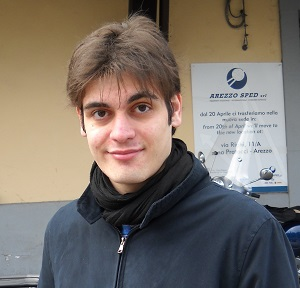
\includegraphics[scale = 0.45]{img/foto_autore.jpg}
  \\
\hline
\end{tabular}


%%% \begin{itemize}
%%% \item Titolo di studio:\\ \\
%%% \item Interessi particolari:\\ \\
%%% \item Ha sostenuto fino ad oggi il seguente numero di esami:\\ \\
%%% \item Deve ancora sostenere i seguenti esami del I anno:\\ \\
%%% \item Prevede di svolgere un tirocinio presso:\\ \\
%%% \item Prevede di laurearsi nella sessione:\\ \\
%%% \item Intende proseguire gli studi per conseguire: \\  \\  \\
%%%   	presso la sede universitaria di: \\ \\
%%% \item Intende entrare subito nel mondo del lavoro presso : \\ \\
%%% \end{itemize}

 
\appendix


\bibliographystyle{abbrv}
\bibliography{biblio}

\end{document}














